\begin{center}

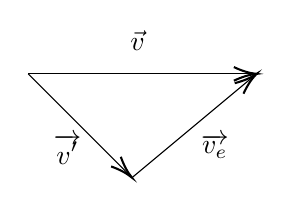
\begin{tikzpicture}[x=0.75pt,y=0.75pt,yscale=-1,xscale=1]
%uncomment if require: \path (0,300); %set diagram left start at 0, and has height of 300

%Straight Lines [id:da7991902571121818] 
\draw    (130,100) -- (238,100) ;
\draw [shift={(240,100)}, rotate = 180] [color={rgb, 255:red, 0; green, 0; blue, 0 }  ][line width=0.75]    (10.93,-3.29) .. controls (6.95,-1.4) and (3.31,-0.3) .. (0,0) .. controls (3.31,0.3) and (6.95,1.4) .. (10.93,3.29)   ;
%Straight Lines [id:da14174806175529686] 
\draw    (130,100) -- (178.59,148.59) ;
\draw [shift={(180,150)}, rotate = 225] [color={rgb, 255:red, 0; green, 0; blue, 0 }  ][line width=0.75]    (10.93,-3.29) .. controls (6.95,-1.4) and (3.31,-0.3) .. (0,0) .. controls (3.31,0.3) and (6.95,1.4) .. (10.93,3.29)   ;
%Straight Lines [id:da019391773911319188] 
\draw    (180,150) -- (238.46,101.28) ;
\draw [shift={(240,100)}, rotate = 140.19] [color={rgb, 255:red, 0; green, 0; blue, 0 }  ][line width=0.75]    (10.93,-3.29) .. controls (6.95,-1.4) and (3.31,-0.3) .. (0,0) .. controls (3.31,0.3) and (6.95,1.4) .. (10.93,3.29)   ;

% Text Node
\draw (178,78) node [anchor=north west][inner sep=0.75pt]   [align=left] {$\displaystyle \vec{v}$};
% Text Node
\draw (141,128) node [anchor=north west][inner sep=0.75pt]   [align=left] {$\displaystyle \overrightarrow{v^{\prime }}$};
% Text Node
\draw (212,128) node [anchor=north west][inner sep=0.75pt]   [align=left] {$\displaystyle \overrightarrow{v_{e}}$};


\end{tikzpicture}

\end{center}